\documentclass[a4paper]{article}

\usepackage{INTERSPEECH2015}

\usepackage[utf8]{inputenc}
\DeclareUnicodeCharacter{0181}{\Ɓ}
\DeclareUnicodeCharacter{0253}{\ɓ}
\DeclareUnicodeCharacter{018A}{\Ɗ}
\DeclareUnicodeCharacter{0257}{\ɗ}
\DeclareUnicodeCharacter{0198}{\Ƙ}
\DeclareUnicodeCharacter{0199}{\ƙ} 

\usepackage{graphicx}
\usepackage{amssymb,amsmath,bm}
\usepackage{textcomp}
\usepackage{hyperref}
\usepackage{subfigure}


\def\vec#1{\ensuremath{\bm{{#1}}}}
\def\mat#1{\vec{#1}}


\sloppy % better line breaks
\ninept

\title{Collaborative Annotation for Person Identification in TV Shows}

\makeatletter
\def\name#1{\gdef\@name{#1\\}}
\makeatother \name{\em Matheuz Budnik$^1$, Laurent Besacier$^1$, Johann Poignant$^2$, Hervé Bredin$^2$, Claude Barras$^2$,  \\
Mickael Stefas$^3$, Pierrick Bruneau$^3$, Thomas Tamisier$^3$}

\address{$^1$Laboratoire d'Informatique de Grenoble (LIG), Univ. Grenoble Alpes, Grenoble, France \\
  $^2$LIMSI, CNRS - Orsay, France \\
  $^3$LIST, Luxembourg \\
  {\small \tt adresses mail} 
}

\begin{document}
  \maketitle
  %
  \begin{abstract}
This paper presents 
  \end{abstract}
  \noindent{\bf Index Terms}: to be added

  \section{Introduction}
      \subsection{Context}
Introduce the Camomile project in general terms. Then IMHO (Pierrick), owing to the space limitations, and for the sake of clarity, we should better restrict the presentation to one of the use cases - as far as the title goes, I guess we should relate to the active learning use case and the dry run experience. 

Resp : all

 \subsection{Demo Content}
The demo shows the shot annotation interface. As for the document structure, I would go the other way: first talk about the use case, and then about the interactive tools to support it. Else we have to talk about a problem that has not been already introduced.

Resp : all

      \section{Collaborative annotation using Camomile tools}

mettre / présenter une vue d'ensemble (schéma) 

Reprendre cette présentation en plus détaillé dans une page github.io 


      \subsection{Collaborative annotation framework}
(présenter le framework et pointer sur le lien github précis - passer rapidement - reprendre anciens articles)

Resp : Johann
  
      \subsection{Web annotation front-end}
%(présenter le front-end web et pointer sur le lien github précis - y passer plus de temps 

% Pierrick: from Mateusz' queue find a more illustrative example, i.e. with context annotation outside the current shot
\begin{figure}[h]
 	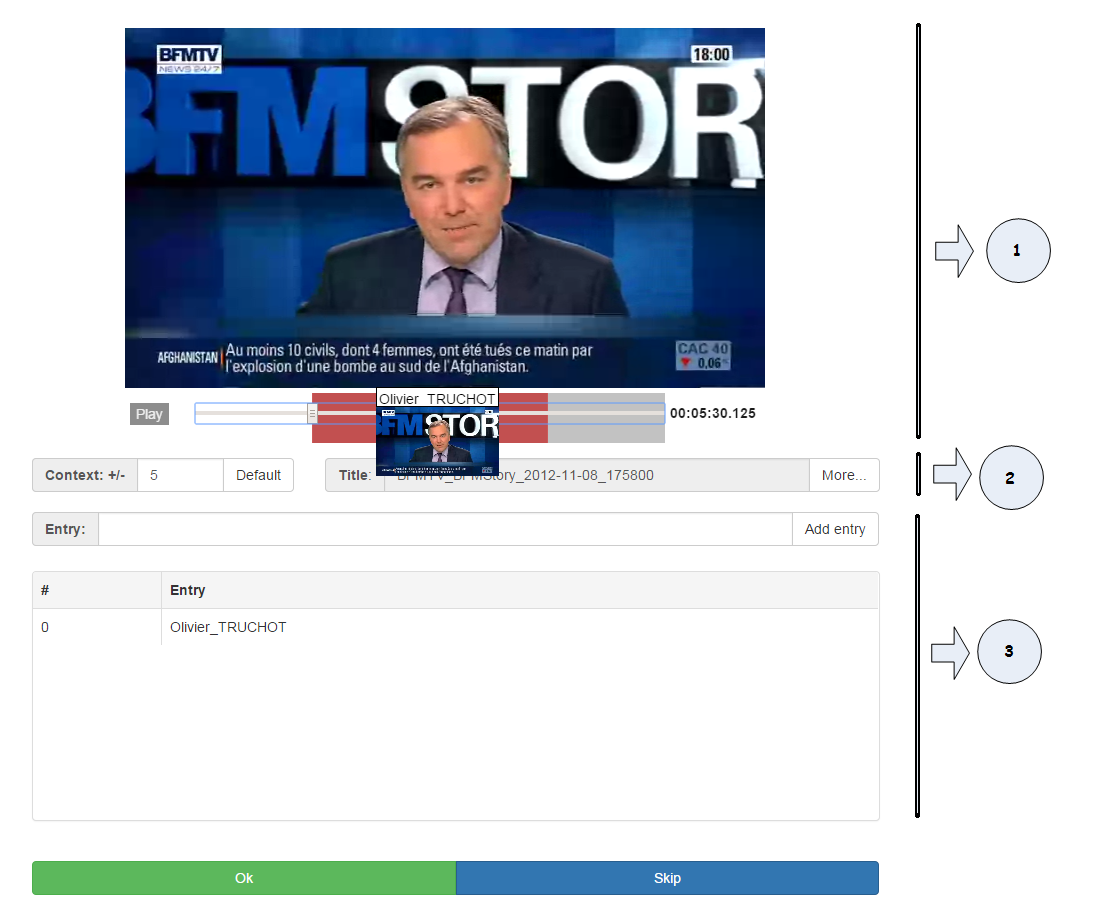
\includegraphics[width=0.5\textwidth]{camomile_ui.png}
	\caption{Overview of the web front-end UI. 1) Video player displaying the shot to annotate and the synchronized \emph{context bar}. 2) The \emph{context bar} configuration and the metadata field. The latter displays the video title, and reveals additional details when activated. 3) The textfield to type the annotation. Multiple annotations are supported, and summarized in a table.}
	\label{fig:frontend}

\end{figure}

% Pierrick: during my trials for the demo video, I found that the annotation list was more annoying than anything else - I has to scroll everytime to do (next), whereas fitting in screen height would make things easier. Also, are multi-annotations to be supported?

An overview of our visual tool is shown in Figure~\ref{fig:frontend}. It heavily uses the display features provided by HTML5 and D3.js \cite{d3js}. The angular.js framework \cite{angularjs} provides an efficient MVC framework to easily coordinate multiple views. The latest version of our tool is available at \cite{urlfrontend}.



Though there are two main use cases, described in Section \ref{sec:shot} and \ref{sec:head}, components are mostly the same for both: the shot or the frame to annotate is displayed in a HTML5 video player and its metadata is shown under the player. The input of a set of annotations is supported by a textfield and a summary table.\\

Both use cases are part of an active learning loop. Each step outputs a selected list of annotations to be performed. Potentially multiple users connect to this list through the frontend, and process annotations in order. They can either validate an annotation of the current shot, or skip it if they feel unsure about it.


% Pierrick: do we talk about both head and shot annotation, or only shot?
\subsubsection{Annotate shot} \label{sec:shot}
In the first use case, a user has to name the speaker in the shot. The player, restricted to the shot, allows to explore it at length.\\
Owing to the iterative nature of the active learning algorithm, the current speaker might have already been annotated elsewhere in the video. Seeking beyond the current shot might reveal such annotations. This obervation led us to propose a \emph{context bar}, which provides the usual features of a seek bar, while revealing annotations performed in previous steps as overlay. A time span can be parametrized around the current shot, highlighted in red (see Figure \ref{fig:frontend}). Hovering over contextual annotations displays a tooltip containing a video thumbnail and the associated annotation.\\

\subsubsection{Annotate head} \label{sec:head}
% Pierrick: did not change anything here for now
The second one corresponds to give the identity of a on screen appearing person. This time, we thought there was no need to scroll through the video, so only the correspong frame is dislayed to the user. As many person can be on screen, we had to help user to figure out which one have to be identified. That's why we add a layer on the frame, on which we drew a red square surronding the head of the right person.\\


%Resp : LIST

      \subsection{Active learning backend}
(présenter l'approche LIG - retraining and adaptation - et pointer sur le lien github précis - y passer plus de temps 

Resp : Matheusz

      \subsection{Compatibility with other annotation tools}
voir si on ajoute une partie comme ça ou pas?

Resp : LIMSI



  \section{Dry run evaluation}
      \subsection{Use case : multimodal speaker annotation}
     
décrire la tâche et les participants à l'expe

Resp : Mateusz
      
      \subsection{Quantitative analysis}
    
stats présentés par Matheusz au meeting de Madrid

Resp : Mateusz
  
     \subsection{Qualitative analysis}
    
%Analyse des resultats du Survey

During the survey, participants had to fill a form to give some  feedback about the web front-end. This was done using Google forms \cite{url-google-forms}. The form is available on \cite{url-list-form}, and the results are visible at \cite{url-list-form-results}.

If the users were mainly satisfied with the front-end, they pointed out some features that have to be improved. As examples, some tooltips or titles had to be added to improve the clarity of the UI, which have already been done since the survey. They also brought up that some component have to be revamped. The "context bar" is an instance of component on which we have to work. As a short term solution, we chose to add the thumbnail displaying a capture of the person concerned by the annotation, but this component will be totally rethought later.
%resp : LIST




  \section{Conclusion}
  
    \subsection{Supporting data files}

description vidéo démo soumise en même temps que le papier
résumé code github pointé ?    

resp : All

    \subsection{Live demo scenario}

décrire précisément ce qui sera présenté à Dresde en Sept 2015

  
  \newpage
  \eightpt
  \bibliographystyle{IEEEtran}
  
  \bibliography{Camomile}

\end{document}
